\section{The Projectmechanism}
\index{Projectmechanism}

OpenCms contains a projectmechanism where all resources exist at least twice -
once for the "Online" project and once for all offline projects. If you 
have enabled versioning, the historic versions of the resources are also 
saved in a separate backup table space.

The projects that can be created with the project management are views on a shared set of offline resources.
If a resource is published, it is copied from the offline space to the online space
and from the online space to the backup (history) space.

\subsection{Data structure}
\index{resources data structure} \index{resources online}
\index{resources offline} \index{resources backup}

There are several tables for the online resources, the offline
resources and the backup resources. This minimizes the quantity of
data in the tables and accelerates queries on the data. Another
advantage is the possiblity to store online, offline and backup
resources on several databases. Each of these three groups has its
own database connection pool.

For the online resources there are the tables
\begin{itemize}
\item CMS\_ONLINE\_RESOURCES
\item CMS\_ONLINE\_FILES
\item CMS\_ONLINE\_PROPERTIES
\item CMS\_ONLINE\_PROPERTYDEF
\end{itemize}

The tables of the online resources are
\begin{itemize}
\item CMS\_RESOURCES
\item CMS\_FILES
\item CMS\_PROPERTIES
\item CMS\_PROPERTYDEF
\end{itemize}

The backup resources are stored in the tables
\begin{itemize}
\item CMS\_BACKUP\_RESOURCES
\item CMS\_BACKUP\_FILES
\item CMS\_BACKUP\_PROPERTIES
\item CMS\_BACKUP\_PROPERTYDEF
\end{itemize}
Each version of a backup resource has a version number. The
information of the project that was published is stored in the
backup tables

\begin{itemize}
\item CMS\_BACKUP\_PROJECT
\item CMS\_BACKUP\_PROJECTRESOURCES.
\end{itemize}

There is another new table named CMS\_PROJECTRESOURCES. This table
contains the ID of a project and the names of the resources that
were selected when the project was created. The entries describe
the view of the project on the offline resources.

\subsection{During installation of OpenCms}

When you setup OpenCms the first time to install the workplace
some data is filled in by default. With regard to the new
projectmechanism

\begin{itemize}
\item the online project is created as permanent project
\item the root folder is created in the online tables
\item the name of the root folder is inserted into the table CMS\_PROJECTRESOURCES for the online project
\item the setup project for the import of the workplace is created as temporary project
\item the root folder is created in the offline tables
\item the name of the root folder is inserted into the table CMS\_PROJECTRESOURCES for the setup project
\end{itemize}

Because the setup project is created by default the setupscript
does not create a project for the import of the workplace.

When the setup project is published the workplace will be copied
to the online tables and to the backup tables. The temporary setup
project will be deleted but the resources still exist in the
offline tables and can be accessed by creating a new project.

\subsection{Creating a new project}
\index{Project permanent}
\index{Project temporary}

A project can be created for permanent or temporary use. A
temporary project will be deleted after it was published.

\begin{figure}[hbt]
\begin{center}
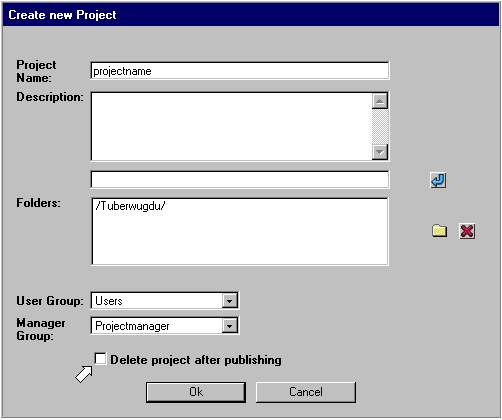
\includegraphics[width=\sgw]
                   {pics/newProject/newPro01}
\caption[Creating a new project]
           {Creating a new project}
\label{newproject}
\end{center}
\end{figure}

When creating a new project only the names of the selected
resources are stored in the new table CMS\_PROJECTRESOURCES and no
resources are copied. So creating a new project is much faster
than before. The new project contains the selected resources and
always the folders \texttt{/system/galleries/pics/}, \texttt{/system/galleries/download/}, \linebreak
\texttt{/system/galleries/externallinks/}, \texttt{/system/galleries/htmlgalleries/} 
and  the folders in \texttt{/system/bodies/} that correspond with the selected folders.

The project is now a view on the offline resources. If two
projects reference the same resource the changes on this resource
will be visible to both projects. If a folder is referenced in
both projects and a new resource is created in this folder in one
project, the new resource is accessible in the other offline project, too.

To avoid that resources that are in work in one project are
published unintentional by another project it is dissuaded from
creating projects that reference the same resources.

\subsection{The view of the project}

The explorer shows all offline resources in an offline project.
The resources that do not belong to the project are grey. The
resources that are referenced by more than one project are
displayed in each of this projects in the same manner: locked
resources with the lock sign, new resources are colored blue,
changed resources are red, deleted resources are crossed out.

If a resource is locked in a project the projectid of this
resource is changed to the current projectid. This is necessary to
guarantee that only the resources that are locked by this project
can be unlocked before they are published.

If you create, delete or change a resource in one project the
changes are immediatly visible to all projects that reference the
resource or one of its subfolders. This behaviour is fundamental
different to the behaviour of the former projectmechanism where
each project has its own version of the resource.

The new, changed or deleted resource gets a little flag. The red
flag means the resources was changed in the current project, the
grey one means the resource was changed in another project.

\subsection{Publish a project}
\index{publish project}

Before a project is published all resources that are locked in
this project are unlocked. Resources that are locked in another
project will be still locked even if they are referenced by the
project that is published.

Only the files and folders in this project that are marked as new,
deleted or changed and that are unlocked will be published.
Resources that were changed and unlocked by another project are
not published.

When a resource is published a copy of this resource is stored in
the backup tables. The versions of a resource in these backup
tables are shown in the \index{history} history of the resource.
The state of the published resource is set to unchanged.

The current information of the published project is stored in a
backup table, too. If the project was created as permanent project
you can go on working in the same project after it is published.
You need not to create a new project as it was required in the
former projectmechanism. A project that was created as temporary
project is deleted and is not accessible any longer.
